\documentclass[12pt]{report}
\usepackage{graphicx}
\usepackage{indentfirst}
\begin{document}
\title{Past to Present Cryptographic Systems Used for Commercial and Personal Purposes}
\author{Sean Connolly\\
The Evergreen State College\\
Methods of Applied Mathematics\\
professorpi@hotmail.com}
\date{\today}
\maketitle
\begin{abstract}
In this paper we will look at several differenct kinds of cryptographic systems, their uses and downfalls (if any).  We will start with a brief introduction on what cryptography is, some of its history and why it is an important thing to know about in this computer filled world we live in.  Then, we will discuss the main concepts of several different types of cryptographic systems, look at the mathematic breakthroughs which has made them possible and look at some simplified examples to see the applications of these newly aquired concepts.
\end{abstract}
\section*{Introduction}

Ever since people have had secrets they have created ways to keep them just that.  During Medival times, writing itself could be seen as a way of keeping secrets.  The only people who where able to read were the rich nobels who could afford a proper education.  They were able to write eachother messages concerning their own affairs and trust that the messenger, even if he did open the message, would not be able to read it.  This was reason enough to keep the peasants illiterate.

Eventually people became smarter and the importance of reading was apparent.  This left people who wanted to hide secrets having to create clever systems for hiding their messages in both wartime and peace.  These, now easily crackable, systems include:  writing messages backwards, Caesar's famous letter shifting cipher, and replacement cyphers.  The point of these systems was to make the messages look like jibberish to someone who was not supposed to read them, but easily readable to the one(s) holding the knowlege of how to decode it.

Ceasar's early shift cipher is simply two concentric cirlces around which the alphabet is written.  For example, to do an a$\rightarrow$e shift the person writing the message whould turn the inside alphabet until the letter a in the inside cirlce lines up with the letter e in the other circle (see figure 1).

\begin{figure}[h]
\centering
\caption{}
\cite{ceaser}

\includegraphics[scale=.3]{ceaser.eps}
\end{figure}

Then the rest of the letters are changed according to their new positions.  Of Course it is easily realized that this method has only 25 different possible keys (the 26th would be plaintext and easily cracked).  Someone who really wanted to read the message could easily go through every possible key in a short amount of time.  We would like to have an encryption system in which the letters are seen as jibberish even if all these 25 keys are used and also impervious to various distribution tests which could give away which letter stands for which. So we need not only a large enough key but also a way that letters could be mapped to two different letters to overcome a letter distribution attack.  There are many systems one could use in which a large number of possible keys could be generated, however in the computer age it is obvious that a computer could go through well over a billion keys per second (government supercomputers may be able to do well over 100 billion per second) forcing our keys to be rather long.  So what would a system look like which is capable of doing all of these things needed to keep the message secret as well as allowing it to be transmitted safely to our friend who we would like to read it? 
\section*{DES}

DES is an acronym for 'Data Encription Standard' and was created so companies had a standardized way in which to encrypt their data and know that it was safe up to a reasonable degree.  DES is what is called a block cipher which means it takes a certain sized chunk of information in the form of bits and transforms it into a non-comprehensible message through a specific algorithm.

More specifically, DES works like this:  First the plaintext message is split up into its binary form and then it is split into blocks of 64 bits (a similiar and safer algorithm would split into 128 or 256 bit blocks but would require a longer key).  The order of these blocks is then rearanged according to the following government created table:

\begin{table}[h]

\begin{center}

\begin{tabular}{ccl}
58  50  42  34  26  18  10  2 &  \\
60  52  44  36  28  20  12  4 &  \\
62  54  46  38  30  22  14  6 &  \\
64  56  48  40  32  24  16  8 &  \\
57  49  41  33  25  17  9   1 &  \\
59  51  43  35  27  19  11  3 &  \\
61  53  45  37  29  21  13  5 &  \\
63  55  47  39  31  23  15  7 &  \\
\end{tabular}

\caption{}\cite{DESalgorithm}

\end{center}

\end{table}

This table mixes up the bits well enough as to protect the message from some known attacks.  It was also later learned that it would fend off other types of attacks not known to the general public when it was created (a hint that the NSA may be aware of much more than they make public)
The inverse of this table which is used later is:

\begin{table}[h]

\begin{center}

\begin{tabular}{ccl}
40  8  48  16  56  24  64  32 &  \\
39  7  47  15  55  23  63  31 &  \\
38  6  46  14  54  22  62  30 &  \\
37  5  45  13  53  21  61  29 &  \\
36  4  44  12  52  20  60  28 &  \\
35  3  43  11  51  19  59  27 &  \\
34  2  42  10  50  18  58  26 &  \\
33  1  41  9   40  17  57  25 &  \\
\end{tabular}

\caption{}\cite{DESalgorithm} 

\end{center}

\end{table}
After the initial mix up, each block then goes through the following algorithm 16 times:
\begin{center}
Ln=Rn-1

Rn=Ln-1 $\rightarrow$ (Rn-1,Kn)
\end{center}

Where R0 is the rightmost bit in the block and L0 is the leftmost bit in the block.  Rn=Ln-1 $\rightarrow$ (Rn-1,Kn) means add L, bit by bit in modulo two from one iteration ago to the term (Rn-1,Kn) where Kn is dependent on the key as such:  Kn=Ks(n, Key).  Where Ks of n is the 'key schedule' found by using another set of government made tables and algorithms.  We will leave the Ks function for interested enough readers to study in their leasure from source \cite{DES} since it is 3-4 pages of rather technical mathematics.  After this algorithm is gone through, the inverse permutation matrix is used and the message is considered hidden.  All which needs to be known about this missing algorithm is that it interweaves the key with the message making them inseparable and therefore difficult to break the ciphertext into its constituent parts.  This makes the only realistic form of attack a brut force, go through all keys attack (although a group of reasearchers have claimed to reduce the number of keys needed to be checked through differential cryptanalysis)$\cite{cracked}$.  

It turns out the inexpensive supercomputers of today are able to crack DES in a matter of hours or even minutes so before a more sophisticated system is agreed upon, larger keys need to be used or else triple-DES could be used.  In triple DES three seperate keys are needed and the entire DES algorithm is done three different times.  This will make your message even safer than it was before, the only draw back is that 3 keys are needed and the computation time is tripled.  Until a better system is chosen however, this is the one to use.

\section*{Public Key Cryptography}
Using DES seems like a very secure system for encrypting your data, but what if we want to send this encrypted data to our friend.  He would have to know the key I used to encrypt it to be able to read it.  This means that I would have to get the key to him somehow.  If we are paranoid enough to have to encrypt this data in the first place, it seems unlikely that we would want to just send the decoding key along the same lines of transmission risking an adversary coming across it.  One way around this would be to have a decided upon code book, but we could never be sure that this isn't copied by someone who we have not given it to and allowing them to silently and easily decrypt any message we send.

Public key cryptography is the way around this problem.  The most useful thing about public key cryptography is that the key which is used to encode the message is different than the one used to decode the message.
\begin{figure}[h]
\centering
\caption{}
\cite{public}
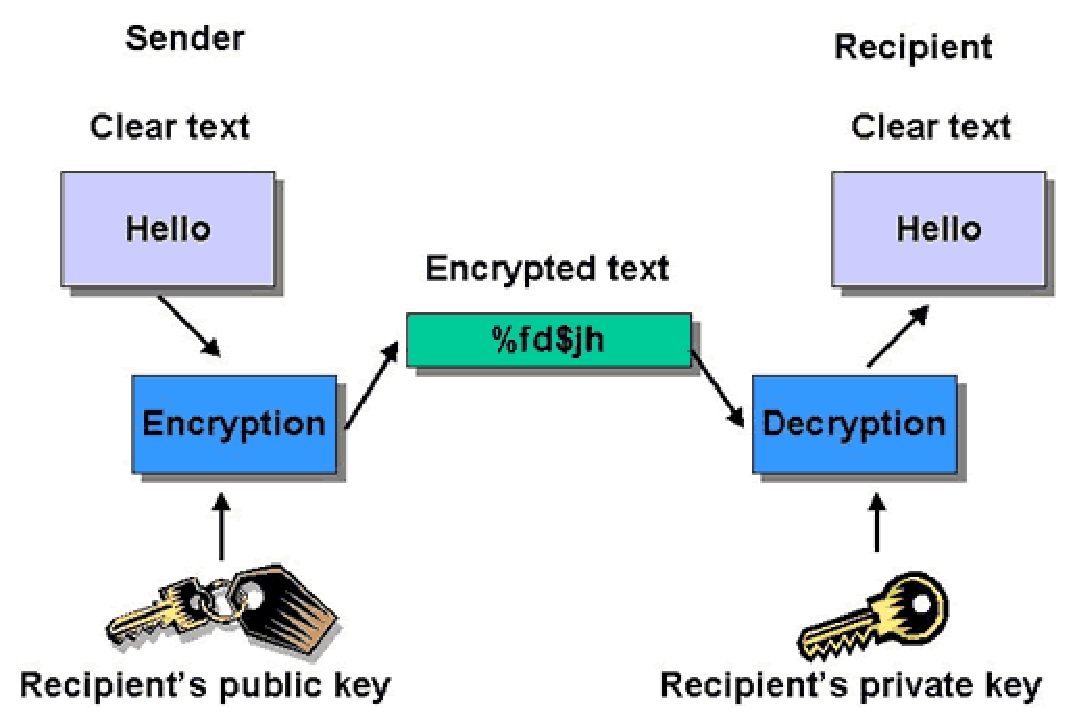
\includegraphics{publickey.eps}
\end{figure}
The creator of the message to be sent finds what is known as 'the reciever's public key'.  The reciever has created this key himself and publishes part of it on his web site or puts it somewhere where all of his friends can see it.  He only makes public, however, the key needed to encode a message to be sent to him and keeps secret the seperate key needed to decode it.  So although anyone can encode a message and send it to him, only he is able to read it.

The algorithm for this particular system is actually rather simple.  First two large prime numbers are chosen 'p' and 'q'.  Then their product is found, 'n'.  After we find their product, we also find $\phi$ which we set to equal (p-1)(q-1).  Then a random integer d is found $\ni 1 < e < \phi$ and the greatest common denominator of $\phi$ and e is 1 (in other words, e is a random prime number less than $\phi$.  After these numbers are all found we calculate d using the extended Euclidean algorithm to compute the uniique integer d, 1$<d<\phi$, $\ni$ ed$\equiv$ 1(mod$\phi$) \cite[page286]{Menezes}.  This algorithm is as follows:\\
\\
\noindent Input:  two non-negative integers a and b with a $\geq$ b.\\
Output:  d-gcd(a,b) and integers x, y satisfying ax+by=d\\
1.  If b=0 then set d$\leftarrow$a, x$\leftarrow$1, y$\leftarrow$0 and return (d,x,y).\\
2.  Set x$_{2}\leftarrow1, x_{1}\leftarrow0, y_{2}\leftarrow0, y_{1}\leftarrow$1.\\
3.  While b$>$0 do the following:\\
3.1  q$\leftarrow$[a/b], r$\leftarrow$a-qb, x$\leftarrow$ x$_{2}-qx_{1}$, y$\leftarrow$y$_{2}-qy_{1}$.\\
3.2  a$\leftarrow b, b\leftarrow r, x_{2}\leftarrow x_{1}, x_{1}\leftarrow x, y_{2}\leftarrow y_{1}, y_{1}\leftarrow$ y.\\
4.  Set d$\leftarrow a, x\leftarrow x_{2}, y\leftarrow y_{2}$ and return (d,x,y).\cite[page 67]{Menezes}
It is easily seen that this is an algorithm a computer could do quite easily.  Now that we have d, our public key is (n,e) and our private key is d.

\noindent Let's look now at a simplified example following the steps above:\\
p=2357\\
q=2551\\
n=pq=6012707
and $\phi$=(p-1)(q-1)=6007800\\
Now we choose a random prime number e=3674911\\
and we find d with the extended Euclidean algorithm (calculations omitted):  d=422191\cite[287]{Menezes}\\

\noindent So our public key is (n=6012707, e=3674911) and the private key is d=422191.  Lets say we have a message m=5234673.  We compute the ciphertext c by c=m$^{e}$mod n = 5234673$^{3674911}$mod 6012707 = 3650502.  This is the message we can now securely send.  Knowing d can you retrieve the plaintext? (Hint: c$^{d}$mod n).

\section*{Electronic Signatures}

Using the new knowledge we now have concerning public key cryptography, we could easily devise a way to create an electonic signature.  Suppose we wanted to ensure that the person I am about to chat with over the internet is actually the friend I want to chat with and not an imposture.  The only way I could be sure of this is if my friend and I both knew something that no one else could possibly no besides us.  Surely my friend's public key wouldn't work because anyone could get it off of his web page and of course he couldn't just show me his private key either (that would defeat the whole purpose).

However, the only thing he has that no one else does is the private key, so that is what we have to utilize.  The easiest way to do this is for me to write a secret message and then encrypt it.  I could then send it to him through our chat room and give him time to put it in his program with his private key to decode it.  Then he could simply repeat the plaintext and I would know that it was him (for who else would be able to decode it?).  

There are more sophisticated ways, of course, to do this but this is surely the simplest.
  
\section*{Conclusion}
We have seen how mathematics is necessary in order to keep secrets secret.  Insight into mathematics can provide clever ways of encrypting data as well as clever ways to decode encrypted data.  Infact, all of the governments of the most powerful nations in the world use a large amount of funds (billions of dollars) to employee mathematicians who's job discription is simply to find ways to encode and decode messages.  These government agencies also have programs set up in order to promote the study of mathematics to ensure that they always have the best mathematicians out af all the industrialized nations or at least the most mathematicians.

DES is a secure system to use in order to encrypt your computer's hard drive or to encrypt personal data which one may not want others to see.  Although it has outlived its life expectancy by over 15 years it is still the primary means of encrypting data these days until a better system comes along.  However it is a rather burdomsome way to send messages to friends, having to deliver the now ever larger keys for them to use as well as the message (which if one bit is out of place becomes unreadible).

Public key cryptography is certainly the most popular way to securely send encrypted messages to friends not having to worry about foes reading it even if you give it directly to them (in order to taunt them).  The clever way of using large primary numbers as keys ensures a safe and nearly uncrackable way to send messages.  Public key cryptography also has the added bonus of allowing one to recieve an electronic signature from a friend in order to varify their identity.  However in a world of ever increacing intelligence among mathematicians it seems to be only a matter of time before this form of cryptography is obsolete and another more sophisticated system takes its place.  We already have inexpensive specially designed computers capable of cracking 128-bit DES in a matter of hours.  It is only a matter of time before someone comes up with a hardware configuration allowing for a quick factorization of a number into its prime pairs making public keys a thing of the past.

\begin{thebibliography} {9}
	\bibitem{Levy}
	  Steven Levy,
	  \emph{Crypto}
	  Viking Penguin, New York,
	  1984.
	\bibitem{Menezes}
	  Alfred J. Menezes, Paul C van Oorshot, and Scott A. Vanstone,
	  \emph{Handbook of Applied Cryptography}
	  CRC Press, New York,
	  1997.
	\bibitem{Mel}
	  Cary Meltzer and Doris Baker,
	  \emph{Cryptography Decrypted}
	  Addison-Wesley, New York,
	  Second Printing
	  2001.
	\bibitem{Simmons}
	  Gustavus J. Simmons,
	  \emph{Contemporary Cryptology, The Science of Information Integrity}
	  IEEE Press, New York,
	  1992.
	\bibitem{ceaser}
	  The Institute for Math and Science Education of the University of Illinois at Chicago,
	  \emph{Cryptography, The Mathematics of Secret Codes}
	  http://cryptoclub.math.uic.edu/about/aboutbook.htm,
	  2004.
	\bibitem{DES}
	  Greg Sterijevski,
	  \emph{The Data E,cryption Standard}
	  http://raphael.math.uic.edu/~jeremy/crypt/contrib/stj.html,
	  Retrieved 2005.
	\bibitem{algorithm}
	  Arnoud Engelfriet,
	  \emph{The DES encryption algorithm}
	  http://www.iusmentis.com/technology/encryption/des/,
	  2003.
	\bibitem{DESalgorithm}
	  Arnoud Engelfriet,
	  \emph{The DES enc,yption algorithm}
	  http://www.itl.nist.gov/fipspubs/fip46-2.htm,
	  2003.
	\bibitem{public}
	  some guy,
	  \emph{public}
	  don't know yet,
	  2003.
	\bibitem{cracked}
	  Dave Rudolf,
	  \emph{Optimized Differential Cryptanalysis of the Data Encryption Standard}
	  University of Saskatchewan, http://davrud.sasktelwebsite.net/programming/des/,
	  2001.
\end{thebibliography}




\end{document}
http://davrud.sasktelwebsite.net/programming/des/